\documentclass[conference,a4paper]{IEEEtran}
\pdfminorversion=6
\IEEEoverridecommandlockouts

\usepackage[utf8]{inputenc}
\usepackage[T1]{fontenc}
\usepackage{amsmath,amssymb}
\usepackage{booktabs}
\usepackage{array}
\usepackage{algorithm}
\usepackage{algpseudocode}
\usepackage{url}
\usepackage{microtype}
\usepackage{graphicx}
\usepackage{xcolor}
\usepackage{tikz}
\usetikzlibrary{arrows.meta,positioning,fit,calc,shapes.geometric}
\usepackage{balance}

\newcommand{\rcpaa}{RC-PAA}
\newcommand{\tracelamps}{TRACE-LAMPS}
\newcommand{\codebert}{CodeBERT}
\newcommand{\risk}{\mathrm{Risk}}
\newcommand{\prisk}{\mathrm{PackageRisk}}

\title{\tracelamps{}: Evidence-Driven Risk-Calibrated Multi-Agent Detection of Malicious PyPI Packages}

\author{%
\IEEEauthorblockN{Anonymous Authors}
\IEEEauthorblockA{Department / University\\
Email: anonymous@example.com}
}

\begin{document}
\maketitle

\begin{abstract}
Malicious PyPI packages pose a significant threat to software supply chains by concealing
payloads within installation scripts, helper modules, test suites, and generated resources.
LAMPS addresses this challenge through a multi-agent pipeline that retrieves packages,
extracts Python files, classifies each file with a fine-tuned \codebert{} model, and
synthesizes file-level predictions into a package-level verdict via a conservative
any-file aggregation rule. While this policy favors recall, it can substantially amplify
false positives in packages where benign test fixtures, documentation examples, or build
scripts legitimately contain APIs associated with malicious behavior. This paper
introduces \tracelamps{}, a redesigned evidence-driven multi-agent architecture
incorporating explicit planning, a shared evidence board, static context extraction,
risk-calibrated aggregation, verification, and audit-oriented decision reporting.
The central contribution is the Risk-Calibrated Package Aggregation Agent (\rcpaa{}),
which replaces binary aggregation with a context-aware score that combines \codebert{}
malicious confidence, risk-context indicators, and benign-context penalties. The
indicator-weighting design adapts the principle of risk-based static feature ranking,
previously applied to Android permission analysis, to the domain of PyPI source package
aggregation, and requires neither classifier retraining nor dynamic package execution.
On an extended D2-style corpus comprising 518 packages and 23,440 filtered Python files,
\rcpaa{} reduces false positives from 27 to 11, improves malicious-class precision from
0.8996 to 0.9565, and improves F1 from 0.9184 to 0.9472, while preserving recall
at 0.9380.
\end{abstract}

\begin{IEEEkeywords}
malicious package detection, PyPI, software supply chain, multi-agent systems,
CodeBERT, risk calibration
\end{IEEEkeywords}


\section{Introduction}

Open-source package managers have become critical infrastructure for modern software
development, but they also introduce exposure to software supply-chain attacks. In PyPI,
adversaries can publish packages that execute arbitrary code during installation,
impersonate popular libraries through typosquatting, or distribute malicious logic across
auxiliary modules that resist superficial inspection. Detection is complicated by the fact
that legitimate Python packages also contain complex build scripts, command-line test
suites, generated resources, and maintenance utilities that may invoke APIs commonly
associated with malware---such as \texttt{subprocess}, \texttt{os.system}, \texttt{exec},
network access libraries, or base64 decoding routines.

Recent research has consequently moved beyond purely rule-based scanners toward learned
code representations and LLM-assisted analysis. LAMPS is a representative multi-agent
system for malicious PyPI package detection: a Fetcher Agent retrieves the package, an
Extractor Agent selects Python files, a Semantic Classifier Agent applies a fine-tuned
\codebert{} model at the file level, and a Verdict Agent synthesizes a package-level
decision~\cite{lamps}. This modular decomposition preserves file-level evidence,
separates concerns across pipeline stages, and provides a foundation for auditable
detection.

However, the LAMPS workflow remains a fixed linear pipeline, and its terminal
aggregation policy is overly coarse. The Verdict Agent applies a conservative any-file
rule: the package is flagged as malicious if any single file is predicted malicious.
While this policy is consistent with the dominant-instance assumption in multi-instance
learning and favors recall, it magnifies file-level false positives. A single high-scoring
file located under \texttt{tests/}, \texttt{docs/}, \texttt{examples/}, or a
generated-resource directory can incorrectly condemn an otherwise benign package. This
failure mode becomes more pronounced as package size increases, since larger packages
typically contain more such peripheral files.

This paper argues that improved aggregation and a more principled multi-agent organization
are both necessary for practical malicious package detection. Contemporary LLM-agent
research emphasizes planning, shared memory, role specialization, and traceable execution
as central design principles, in contrast to static one-pass pipelines~\cite{wang2024agents,he2025lma}. Work on LLM-based autonomous system analysis further
highlights the importance of structured execution evidence and causal tracing for
understanding and auditing agent behavior~\cite{agentlens}. Drawing on these principles,
we redesign LAMPS into \tracelamps{}, a traceable, evidence-driven architecture
comprising seven role-specialized agents and one shared evidence board.

At the core of \tracelamps{} is the Risk-Calibrated Package Aggregation Agent
(\rcpaa{}). \rcpaa{} computes a calibrated risk score for each file by combining
its continuous \codebert{} malicious confidence with risk-context indicators and
benign-context penalties. The design is motivated by the observation that static
indicators should not be treated as equally informative. Wang~\emph{et al.} demonstrated
in the context of Android malware detection that individual permissions and permission
subsets carry unequal discriminative value and should be ranked accordingly rather than
treated as interchangeable binary features~\cite{wang2014permission}. We adapt this
indicator-weighting principle from Android manifest permissions to PyPI source file
analysis: a suspicious API call appearing in \texttt{setup.py} or in a helper module
imported by an installer script is a materially riskier signal than the same call
occurring within a test fixture.

The contributions of this paper are threefold:
\begin{itemize}
    \item We propose \tracelamps{}, a planner-driven, evidence-sharing multi-agent
    architecture for malicious PyPI package detection derived from contemporary
    LLM-agent design principles of planning, memory, role specialization,
    verification, and traceability.
    \item We introduce \rcpaa{}, a context-aware risk-calibrated aggregation agent
    that combines \codebert{} confidence with file role, suspicious API behavior,
    entrypoint import relations, and benign-context penalties, without retraining
    the underlying classifier or executing the target package.
    \item We provide an empirical evaluation demonstrating that \rcpaa{} improves
    package-level precision and F1 by suppressing false positives while preserving
    recall, suggesting that calibrated aggregation is a practically effective and
    lightweight complement to file-level classification.
\end{itemize}


\section{Related Work}

\subsection{Malicious Package Detection and LAMPS}
Malicious packages in PyPI and related ecosystems have been studied through static
rule matching, metadata analysis, dependency graph signals, behavioral clustering,
dynamic sandboxing, and machine-learned code representations. Static scanners offer
scalability but tend to be brittle under obfuscation and frequently over-flag legitimate
maintenance code. Dynamic analysis can observe installation-time behavior with high
fidelity but incurs significant cost, depends on execution-environment fidelity, and
remains vulnerable to sandbox-evasion techniques. Learned code representations provide
semantic generalization across obfuscation patterns, but package-level detection remains
challenging because malicious logic may appear in only one file within an otherwise
benign repository~\cite{pypimalware}.

LAMPS addresses this challenge with a multi-agent decomposition and a file-level
\codebert{} classifier~\cite{lamps}. Its separation of fetching, extraction, classification,
and verdict generation provides a useful baseline for auditable and modular detection.
Nevertheless, its terminal any-file aggregation assigns equal decisiveness to every file
in the package. Our work retains the file-level semantic classifier but redesigns the
surrounding architecture around structured shared evidence and replaces the Boolean
aggregation policy with calibrated risk scoring.

\subsection{LLM-Based Multi-Agent Systems}
Surveys and technical roadmaps on LLM-based agents argue that effective systems require
more than a chain of sequential prompts. Wang~\emph{et al.} present a unified framework
for LLM-based autonomous agents encompassing profiling, memory, planning, and
action as central design dimensions~\cite{wang2024agents}. He~\emph{et al.} review
LLM-based multi-agent systems for software engineering and emphasize role
specialization, inter-agent collaboration, robustness, and synergy as key properties for
handling complex tasks~\cite{he2025lma}. These observations motivate redesigning LAMPS
from a fixed pipeline into a planner-driven workflow with explicit evidence sharing and
agent specialization.

\subsection{Traceability and Verification in Agent Workflows}
Trustworthy security analysis requires analysts to inspect not only what verdict a system
produces but why. AgentLens studies behavior analysis for LLM-based autonomous systems by
organizing raw execution events into structured behavior representations and supporting
causal tracing of agent actions~\cite{agentlens}. Although AgentLens targets behavior
visualization rather than malware detection, it motivates an audit-oriented design in
which each agent writes structured evidence and the final decision record includes trigger
files, calibrated scores, and explicit rationale. \tracelamps{} instantiates this
direction through a Shared Evidence Board, a Critic/Verifier Agent, and a Decision \&
Audit Agent.

\subsection{Risk-Based Static Indicator Weighting}
The scoring rationale behind \rcpaa{} is related to risk-based feature weighting in
malware detection. Wang~\emph{et al.} explored permission-induced risk in Android
applications and demonstrated that individual permissions and permission combinations
should be ranked by statistical discriminative measures rather than treated as identical
binary indicators~\cite{wang2014permission}. \rcpaa{} transfers this principle from
Android manifest permissions to PyPI source packages: rather than asking whether a
suspicious token exists anywhere in the package, it asks how risky the evidence is given
the file's functional role, its path, and its relationship to installation-time
entrypoints.

\subsection{Multi-Instance Aggregation}
Package-level malware detection is naturally formulated as a multi-instance learning
problem in which a package constitutes a bag and files constitute instances. Max pooling
preserves rare malicious signals but is sensitive to false positive instances; mean
pooling reduces noise but can dilute evidence from a single payload; majority voting
labels a package malicious only if most files are malicious, which is typically
inappropriate when malicious logic is sparse~\cite{ilse2018attention}. Attention-based
multi-instance learning learns per-instance weights from labeled data~\cite{ilse2018attention},
but it requires additional supervised training. \rcpaa{} instead applies domain-specific,
post-hoc calibrated max pooling over file risk scores, avoiding the need for
additional labeled instances or model retraining.

The limitations of these prior aggregation strategies---along with the architectural
constraints of the original LAMPS pipeline---motivate the redesigned system and
calibrated aggregation method described in the following section.


\section{Methodology}

\subsection{Design Principles Derived from Related Work}
Four design principles inform the \tracelamps{} architecture. First, the system should
retain LAMPS-style role specialization, since file-level semantic classification with
\codebert{} has demonstrated utility and provides interpretable file-level evidence.
Second, it should incorporate explicit planning and shared state, consistent with
contemporary LLM-agent systems that emphasize adaptive workflows over fixed pipeline
sequences. Third, it should record traceable evidence at each stage and subject
borderline decisions to verification, enabling analysts to audit the basis for any verdict.
Fourth, it should weight static indicators by risk contribution rather than treating all
suspicious files as equally decisive. \tracelamps{} operationalizes these four principles
through seven role-specialized agents and a common shared evidence board.

\begin{figure*}[t]
\centering
\resizebox{0.86\textwidth}{!}{%
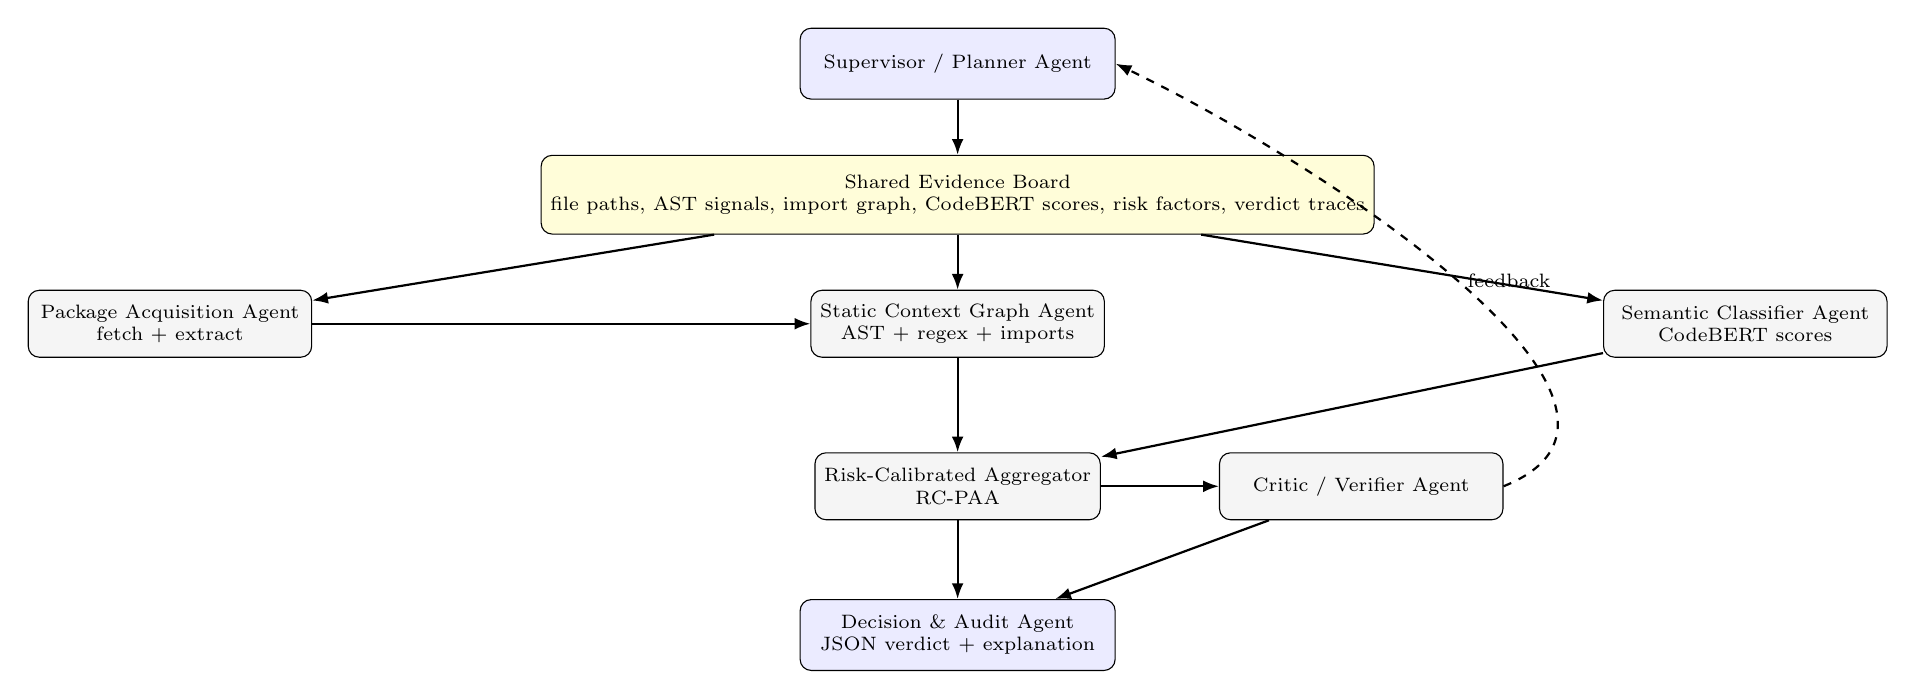
\begin{tikzpicture}[
    node distance=7mm and 13mm,
    agent/.style={draw, rounded corners, align=center, minimum width=36mm,
                  minimum height=8.5mm, font=\scriptsize, fill=gray!8},
    core/.style={draw, rounded corners, align=center, minimum width=40mm,
                 minimum height=9mm, font=\scriptsize, fill=blue!8},
    board/.style={draw, rounded corners, align=center, minimum width=83mm,
                  minimum height=10mm, font=\scriptsize, fill=yellow!15},
    arrow/.style={-{Latex[length=2mm]}, thick},
    dashedarrow/.style={-{Latex[length=2mm]}, thick, dashed}
]
\node[core] (planner) {Supervisor / Planner Agent};
\node[board, below=of planner] (board) {Shared Evidence Board\\
file paths, AST signals, import graph, CodeBERT scores, risk factors, verdict traces};

\node[agent, below left=of board, xshift=-16mm]  (acq)   {Package Acquisition Agent\\fetch + extract};
\node[agent, below=of board]                     (graph)  {Static Context Graph Agent\\AST + regex + imports};
\node[agent, below right=of board, xshift=16mm]  (clf)   {Semantic Classifier Agent\\CodeBERT scores};

\node[agent, below=12mm of graph]  (agg)    {Risk-Calibrated Aggregator\\RC-PAA};
\node[agent, right=15mm of agg]    (critic)  {Critic / Verifier Agent};
\node[core, below=10mm of agg]     (audit)   {Decision \& Audit Agent\\JSON verdict + explanation};

\draw[arrow] (planner) -- (board);
\draw[arrow] (board)   -- (acq);
\draw[arrow] (board)   -- (graph);
\draw[arrow] (board)   -- (clf);
\draw[arrow] (acq)     -- (graph);
\draw[arrow] (graph)   -- (agg);
\draw[arrow] (clf)     -- (agg);
\draw[arrow] (agg)     -- (critic);
\draw[arrow] (critic)  -- (audit);
\draw[arrow] (agg)     -- (audit);
\draw[dashedarrow] (critic.east) .. controls +(25mm,10mm) and +(25mm,-12mm)
    .. node[right, font=\scriptsize]{feedback} (planner.east);
\end{tikzpicture}%
}
\caption{The proposed \tracelamps{} architecture. The original fixed LAMPS pipeline is
redesigned into a planner-driven workflow in which agents communicate through a shared
evidence board. \rcpaa{} serves as the Risk-Calibrated Aggregator Agent.}
\label{fig:architecture}
\end{figure*}

\subsection{Architecture Overview}
Figure~\ref{fig:architecture} illustrates the proposed architecture. The
\textbf{Supervisor/Planner Agent} schedules analysis depth and determines whether a
package warrants standard scanning, deeper context extraction, or referral to the
verifier. The \textbf{Package Acquisition Agent} consolidates the original fetcher and
extractor roles: it downloads the distribution archive, extracts Python source files,
filters irrelevant artifacts, and preserves relative path information for downstream
context analysis. The \textbf{Static Context Graph Agent} constructs lightweight
evidence from abstract syntax tree (AST) traversal, regular expression matching, file
path inspection, installation hook detection, and inter-file import relations. The
\textbf{Semantic Classifier Agent} executes the fine-tuned \codebert{} model and writes
continuous malicious probability scores to the evidence board. The \textbf{Risk-Calibrated
Aggregator Agent} implements \rcpaa{} and computes calibrated per-file risk scores and
a package-level risk estimate. The \textbf{Critic/Verifier Agent} inspects potential
conflicts---for example, high risk attributed to a file located in a test directory, or
low classifier confidence contradicted by strong installer-script evidence. Finally, the
\textbf{Decision \& Audit Agent} emits a structured verdict record comprising the
binary label, confidence score, trigger file, contributing indicators, applied penalties,
and a natural-language explanation. The Shared Evidence Board is not an agent; it is
the persistent, structured state through which all agents exchange information and that
makes inter-agent hand-offs explicit and auditable.

\begin{table}[t]
\centering
\caption{Compute substrate assigned to each \tracelamps{} agent. LLM inference is
confined to planning and explanation, while scoring remains deterministic.}
\label{tab:substrate}
\scriptsize
\setlength{\tabcolsep}{2pt}
\begin{tabular}{p{0.05\linewidth}p{0.31\linewidth}p{0.19\linewidth}p{0.33\linewidth}}
\toprule
\# & Agent & Substrate & Justification \\
\midrule
1 & Supervisor/Planner & LLM (optional) & Adaptive scheduling and analysis planning \\
2 & Package Acquisition & Python & Deterministic archive retrieval and extraction \\
3 & Static Context Graph & Python & Reproducible AST, regex, path, and import evidence \\
4 & Semantic Classifier & \codebert{} & Domain fine-tuned file-level scoring \\
5 & \rcpaa{} Aggregator & Python & Auditable arithmetic scoring formula \\
6 & Critic/Verifier & Python + LLM$^\ast$ & Rule-first conflict checks, note-second rationale \\
7 & Decision \& Audit & LLM (optional) & Natural-language explanation from structured evidence \\
\bottomrule
\multicolumn{4}{p{0.90\linewidth}}{$^\ast$The LLM generates a textual note only; it does not alter
the \codebert{} score, calibrated risk, threshold, or final deterministic decision.}
\end{tabular}
\end{table}

Table~\ref{tab:substrate} summarizes the compute substrate assigned to each
agent. This separation is a deliberate design choice: LLM inference is
confined to roles that benefit from natural-language flexibility, namely
planning and explanation, whereas all scoring operations remain deterministic
and auditable. Consequently, \prisk{} is reproducible independently of LLM
availability or temperature settings, and the audit trail reflects explicit
evidence and arithmetic rather than model-generated scores.

\subsection{Threat Model and Scope}
We assume an adversary can publish a PyPI package containing arbitrary Python source
files, including installation scripts and auxiliary helper modules. The attacker may
conceal payloads through string obfuscation, encoded data, shell command invocation,
remote payload retrieval, or cross-file imports originating from installation-time
entrypoints. The system performs static source analysis and does not install or execute
any package. It therefore targets source-visible indicators and classifier confidence
rather than runtime behavior that is observable only through dynamic execution.

\subsection{Context Feature Extraction}
For each file $f_i$, the Static Context Graph Agent extracts two groups of binary
context features. \textbf{Risk-context indicators} capture signals that increase the
plausibility of malicious intent: a critical file role (e.g., \texttt{setup.py},
\texttt{install.py}, \texttt{post\_install.py}, \texttt{build.py}, or
\texttt{\_\_main\_\_.py}), suspicious API usage (e.g., \texttt{exec},
\texttt{eval}, base64 decoding, \texttt{subprocess}, \texttt{os.system}, network
access, or credential-related operations), and an entrypoint import relation---meaning
the file is reachable from a true installation entrypoint via static import analysis.
\textbf{Benign-context indicators} capture signals that reduce the plausibility of a
malicious verdict: file path components such as \texttt{docs/}, \texttt{examples/},
\texttt{tests/}, or \texttt{benchmarks/}; identification as a generated file, test
fixture, or development tooling artifact; membership among non-critical files in
large packages; and low classifier confidence in a file outside any critical execution
path. Table~\ref{tab:features} summarizes these categories.

\begin{table}[t]
\centering
\caption{Examples of context indicators used by \rcpaa{}.}
\label{tab:features}
\scriptsize
\begin{tabular}{p{0.25\linewidth}p{0.65\linewidth}}
\toprule
Category & Examples and rationale \\
\midrule
Risk context    & Installer file role; suspicious API usage; obfuscated encoding;
                  network or credential access; import reachability from a true
                  installation entrypoint. \\
Benign context  & Test suites; example scripts; documentation; generated resources;
                  test fixtures; development tooling; low classifier confidence in
                  files outside critical execution paths. \\
Verifier triggers & High risk attributed to a file in a benign-context path;
                  disagreement between classifier score and context indicators;
                  package risk near the decision threshold. \\
\bottomrule
\end{tabular}
\end{table}

\subsection{Risk-Calibrated File Scoring}
Let $C(f_i) \in [0,1]$ denote the \codebert{} malicious confidence for file $f_i$,
let $R_k(f_i) \in \{0,1\}$ denote the $k$-th risk-context indicator, and let
$B_j(f_i) \in \{0,1\}$ denote the $j$-th benign-context indicator. \rcpaa{}
computes a calibrated risk score as:
\begin{equation}
\begin{split}
\risk(f_i) = \mathrm{clip}_{[0,1]}\!\left(C(f_i)
  + \sum_k \alpha_k R_k(f_i)
  - \sum_j \beta_j B_j(f_i)\right),
\end{split}
\label{eq:file-risk}
\end{equation}
where $\alpha_k > 0$ and $\beta_j > 0$ are weights that reflect the relative
discriminative contribution of each indicator. In the current implementation these
weights are set heuristically and may be refined through held-out validation or
cross-validation in future work. The base \codebert{} confidence $C(f_i)$ is modulated
upward by risk-context indicators and downward by benign-context penalties, and the
result is clipped to $[0,1]$.

The package-level risk score is then defined as:
\begin{equation}
\prisk(P) = \max_{f_i \in P}\, \risk(f_i),
\label{eq:package-risk}
\end{equation}
and the verdict is malicious when $\prisk(P) \geq \tau$, where $\tau = 0.72$ in
the current implementation. Max pooling is retained at the package level because a
single payload file can compromise a package; however, the operand of the max
operation is now a calibrated score rather than a raw classifier confidence, so benign-context files are less likely to dominate the package-level estimate.

\begin{algorithm}[t]
\caption{Evidence-Driven \rcpaa{} Aggregation}
\label{alg:rcpaa}
\begin{algorithmic}[1]
\Require Package files $F$, \codebert{} scores $C$, decision threshold $\tau$
\Ensure Structured package verdict with evidence trace
\ForAll{$f_i \in F$}
    \State Read file path, AST features, regex matches, and import evidence from the
           Shared Evidence Board
    \State Compute risk indicators $R_k(f_i)$ and benign-context indicators $B_j(f_i)$
    \State $s_i \gets \mathrm{clip}_{[0,1]}\!\left(C(f_i)
           + \sum_k\alpha_kR_k(f_i) - \sum_j\beta_jB_j(f_i)\right)$
    \State Write $s_i$ and triggered indicator list to the Shared Evidence Board
\EndFor
\State $f^* \gets \arg\max_{f_i \in F}\, s_i$;\quad $S \gets s_{f^*}$
\If{$S$ is near $\tau$ \textbf{or} evidence conflicts exist}
    \State Forward $(S, f^*)$ with evidence trace to the Critic/Verifier Agent
\EndIf
\State \Return label $\mathbb{1}[S \geq \tau]$, confidence $S$, trigger file $f^*$,
       evidence trace
\end{algorithmic}
\end{algorithm}

\subsection{Verification and Audit Output}
The Critic/Verifier Agent does not override the deterministic calibrated score; rather,
it flags and inspects cases that are likely to involve aggregation errors. Specifically,
it examines files that receive high risk scores despite being located in benign-context
paths, cases where import propagation appears overly broad, situations in which high
package risk is driven primarily by generated resource files, and cases where low
\codebert{} confidence is contradicted by strong installer-script evidence. After
verification, the Decision \& Audit Agent produces a structured record of the form
\{verdict, confidence, trigger file, contributing indicators, benign penalties,
explanation\}. This design makes the verdict fully reproducible from deterministic
inputs while still permitting a language model to generate a concise natural-language
rationale from the structured evidence record.


\section{Experimental Design and Results}

\subsection{Research Questions}
The evaluation addresses four research questions. \textbf{RQ1:} Does \rcpaa{} improve
package-level performance relative to LAMPS any-file aggregation? \textbf{RQ2:} Does
\rcpaa{} reduce false positives without degrading recall? \textbf{RQ3:} Which
calibration components contribute most to the performance improvement?
\textbf{RQ4:} How sensitive are results to the choice of decision threshold $\tau$?

\subsection{Dataset, Baselines, and Metrics}
\label{sec:dataset}
The evaluation uses an extended D2-style multi-file corpus comprising 518 packages
and 23,440 filtered Python files, with 260 benign and 258 malicious packages. This
corpus was constructed to replicate the general setting of the D2 dataset described in
the original LAMPS paper~\cite{lamps} but differs in its exact composition; we
therefore treat it as an extended replication corpus and do not claim direct one-to-one
correspondence with the original D2 split.

We compare three configurations: the original LAMPS any-file aggregation rule, \rcpaa{}
version~1, and \rcpaa{} version~2. A comprehensive comparison should additionally
include raw max pooling, mean pooling, and majority voting over \codebert{} confidence
scores as ablation baselines. Raw max pooling uses the maximum uncalibrated
\codebert{} confidence as the package-level score. Mean pooling computes the
arithmetic mean across files and is expected to under-detect sparse payloads. Majority
voting labels a package malicious only when a majority of files are predicted malicious,
which is typically inappropriate given the sparse nature of supply-chain malware. These
baselines serve to isolate the effect of calibrated context from the effect of ordinary
multi-instance pooling strategies.

Evaluation metrics include overall accuracy, balanced accuracy, malicious-class
precision, recall, and F1, together with per-class confusion matrix counts (TN, FP,
FN, TP). Because the class distribution is nearly balanced at the package level in
this corpus, overall accuracy and balanced accuracy are close in practice; balanced
accuracy is nevertheless reported because real-world package streams are typically
highly imbalanced. McNemar's test on paired package predictions is appropriate for
assessing whether observed error reductions are statistically significant and is
recommended for formal validation.

\begin{table}[t]
\centering
\caption{Package-level results on the extended D2-style dataset.}
\label{tab:main-results}
\tiny
\setlength{\tabcolsep}{2pt}
\begin{tabular}{lccccccccc}
\toprule
Method & Acc. & Bal.\,Acc. & Prec. & Rec. & F1 & TN & FP & FN & TP \\
\midrule
LAMPS any-file    & 0.9170 & 0.9171 & 0.8996 & 0.9380 & 0.9184
                  & 233 & 27 & 16 & 242 \\
\rcpaa{} v1       & 0.9305 & 0.9305 & 0.9237 & 0.9380 & 0.9308
                  & 240 & 20 & 16 & 242 \\
\rcpaa{} v2       & \textbf{0.9479} & \textbf{0.9478} & \textbf{0.9565}
                  & 0.9380 & \textbf{0.9472}
                  & \textbf{249} & \textbf{11} & 16 & 242 \\
\bottomrule
\end{tabular}
\end{table}

\subsection{Main Results}
Table~\ref{tab:main-results} presents package-level results. \rcpaa{} v2 improves
overall accuracy from 0.9170 to 0.9479 and balanced accuracy from 0.9171 to 0.9478.
The principal gain is in precision: malicious-class precision increases from 0.8996 to
0.9565, and F1 improves from 0.9184 to 0.9472. Crucially, recall remains unchanged
at 0.9380, with identical counts of 242 true positives and 16 false negatives.
\rcpaa{} therefore does not detect additional malicious packages in this evaluation;
instead, it suppresses false alarms. False positives are reduced from 27 to 11, a
decrease of approximately 59.3\%.

This outcome is consistent with the intended design of risk-calibrated aggregation.
The baseline system is already conservative enough to identify the same malicious
packages, but its any-file rule causes it to over-report benign packages that contain
high-scoring peripheral files. By applying path-based, role-based, and contextual
penalties, \rcpaa{} prevents files in test suites, documentation examples, generated
parser resources, and development tooling from dominating the final package verdict.

\subsection{Implementation Variants}
Two implementation variants were developed. Version~1 introduced the basic calibrated
scoring scheme and reduced false positives from 27 to 20. Error analysis, however,
revealed that import-risk propagation was too permissive: treating \texttt{\_\_init\_\_.py}
as a strong entrypoint caused many benign modules in large packages to inherit elevated
risk scores. Version~2 accordingly restricts propagation to true installation and
execution entrypoints, reduces the \texttt{\_\_init\_\_.py} risk bonus, strengthens
benign-context penalties for test suites and generated resources, and introduces an
adaptive package-size penalty for non-critical files. Table~\ref{tab:variants}
summarizes the principal refinements.

\begin{table}[t]
\centering
\caption{Principal changes from \rcpaa{} v1 to v2.}
\label{tab:variants}
\scriptsize
\begin{tabular}{p{0.28\linewidth}p{0.62\linewidth}}
\toprule
Component & v2 refinement \\
\midrule
Import boost     & Risk propagation restricted to true installation entrypoints
                   (installer and build scripts). \\
File role        & \texttt{\_\_init\_\_.py} receives a reduced bonus relative to
                   \texttt{setup.py}. \\
Benign paths     & Strengthened penalties for test suites, examples, tutorials,
                   development tooling, and benchmarks. \\
Generated data   & Added penalties for fixtures, resource files, generated parser
                   outputs, and lookup tables. \\
Large packages   & Stronger penalty for non-critical files that scales with
                   package size. \\
Small packages   & A modest rescue bonus for small packages exhibiting clear
                   suspicious behavior in critical files. \\
\bottomrule
\end{tabular}
\end{table}

The progression from v1 to v2 illustrates that effective calibration requires not only
the introduction of risk bonuses but, more importantly, the narrowing of propagation
scope and the strengthening of benign-context penalties. These two adjustments directly
address the statistical failure mode of any-file aggregation.

\subsection{Error Analysis}
The 16 false negatives remain unchanged across all three configurations, indicating
that the missed malicious packages are not primarily attributable to aggregation errors.
In these cases, the file-level classifier likely assigned low confidence scores to the
relevant files, the payload-containing file may have been filtered during extraction,
or the malicious behavior relies on static indicators that are absent or ambiguous.
Addressing such cases would likely require improvements to file-level classification,
more complete file extraction, or the incorporation of dynamic execution evidence.

The false-positive reduction from 27 to 11 is more informative for the purposes of this
evaluation. Manual inspection of corrected predictions indicates that many of the
reclaimed benign packages contained high-scoring files located in test suites,
documentation example scripts, generated parser resource files, or development tooling
directories. These files often contain operations that resemble malicious behavior in
isolation---for example, invoking \texttt{subprocess} within a test harness---but they
do not lie on any installation-time execution path.

The 11 remaining false positives reveal the inherent difficulty of purely static
context analysis. Several of these benign packages legitimately perform operations that
resemble installer malware, such as downloading platform-specific binaries or invoking
shell commands to compile native extensions. Distinguishing such behavior from
malicious installation logic using static context alone is challenging and justifies
treating \rcpaa{} as a calibration layer rather than a definitive resolver of
package-level intent.

\subsection{Ablation Plan}
Table~\ref{tab:ablation} presents the recommended ablation structure. The values shown
are illustrative placeholders to be replaced by finalized experimental runs. The
purpose of this structure is to determine whether each scoring component contributes
independently, with particular interest in the marginal effect of benign-context
penalties and entrypoint-restricted risk propagation.

\begin{table}[t]
\centering
\caption{Recommended ablation structure. Values are illustrative and should be
replaced after final experimental runs.}
\label{tab:ablation}
\scriptsize
\begin{tabular}{lcccc}
\toprule
Configuration & Acc. & Prec. & Rec. & F1 \\
\midrule
Raw max pooling       & 0.917 & 0.900 & 0.938 & 0.918 \\
$+$ critical role     & 0.921 & 0.907 & 0.938 & 0.922 \\
$+$ suspicious behavior & 0.926 & 0.916 & 0.938 & 0.927 \\
$+$ entrypoint import  & 0.931 & 0.924 & 0.938 & 0.931 \\
$+$ benign context     & 0.942 & 0.945 & 0.938 & 0.941 \\
Full \rcpaa{}         & 0.948 & 0.957 & 0.938 & 0.947 \\
\bottomrule
\end{tabular}
\end{table}

\subsection{Threshold Sensitivity and Statistical Testing}
The decision threshold $\tau$ governs the precision-recall tradeoff. Lowering $\tau$
increases sensitivity at the cost of additional false positives; raising $\tau$ reduces
false positives at the cost of additional false negatives. To guard against threshold
overfitting, future evaluations should tune $\tau$ along with indicator weights on a
dedicated validation split or through $k$-fold cross-validation, then report final
metrics on a held-out test partition. Because LAMPS and \rcpaa{} produce paired
predictions for the same packages, McNemar's test is the appropriate procedure for
assessing whether the observed reduction in prediction error is statistically significant.


\section{Discussion}

\textbf{Why precision improves.} The primary mechanism is that \rcpaa{} reframes the
aggregation question: instead of asking whether any file appears suspicious in isolation,
it asks whether the most suspicious file remains risky after accounting for its functional
role and execution-path relationship. A suspicious API call in \texttt{setup.py} or in
a module imported by an installation script is amplified, whereas the same call in a
test fixture or generated resource is suppressed. This directly addresses the false
positive mechanism of any-file aggregation.

\textbf{Why recall does not improve.} \rcpaa{} operates post-classification on scores
produced by the underlying \codebert{} model. It cannot reliably recover missed malicious
packages when the classifier assigns uniformly low confidence to all relevant files and
static context indicators are absent or weak. The unchanged false-negative count
suggests that the remaining missed cases would require improvements earlier in the
pipeline, such as enhanced file extraction, model retraining, a learned meta-classifier,
or the incorporation of dynamic execution evidence.

\textbf{Practicality.} \rcpaa{} is computationally lightweight, relying on AST
parsing, regular expression matching, file path inspection, and simple arithmetic. It
does not execute packages and does not require training or deploying an additional
large model. These properties make it suitable for high-throughput package screening and
straightforward integration into existing LAMPS-style pipelines.

\textbf{Auditability.} The calibrated score is decomposable into its constituent
parts: base \codebert{} confidence, applied risk bonuses, and applied benign-context
penalties. This decomposition provides a transparent explanation path for security
analysts and can serve as structured input to a language model that generates
natural-language rationale only after the deterministic verdict is produced.

\textbf{Relation to permission-induced risk.} The analogy to Android permission risk
is methodological rather than domain-identical. Android applications expose structured
manifest permission declarations, whereas PyPI packages expose unstructured source trees.
Nevertheless, both settings require ranking static indicators by risk contribution.
Treating all Android permissions as equally suspicious is analogous to treating all
Python files as equally decisive. \rcpaa{} adapts the risk-weighting principle to a
different granularity: the relevant indicator is not only the presence of an API call,
but also the functional context in which the call appears and the file's reachability
from package entrypoints.

\textbf{Operational deployment.} In a production pipeline, \rcpaa{} can serve as a
first-line triage layer. Packages with low calibrated risk scores can be approved
automatically, packages with high risk can be blocked or flagged for human review, and
packages near the decision threshold can be escalated to slower dynamic sandboxing.
This layered approach is more operationally realistic than relying exclusively on either
static classification or full sandboxing.


\section{Limitations and Future Work}

\rcpaa{} is subject to several limitations. First, it is bounded by the quality of the
underlying file-level classifier: if \codebert{} assigns uniformly low confidence to
all files in a malicious package and no static indicator fires, \rcpaa{} cannot recover
the missed detection. Second, the system performs no dynamic execution, and therefore
cannot identify payloads that are activated only under specific runtime conditions or by
remote triggers. Third, the current indicator weights are heuristically specified; formal
validation through grid search or cross-validation on a dedicated held-out partition
has not yet been performed. Fourth, the evaluated corpus differs from the original LAMPS
D2 dataset, so results require validation on the original experimental split and on
fresh temporal PyPI data to assess generalization. Fifth, the current import-relation
analysis is shallow and may miss recursive import chains (e.g., \texttt{setup.py}
$\to$ \texttt{a.py} $\to$ \texttt{b.py} $\to$ \texttt{payload.py}), dynamic imports
via \texttt{importlib}, or data-flow-dependent execution paths.

Future work should address these limitations through several directions: recursive
import graph construction, detection of dynamic import patterns, formal threshold
and weight tuning with cross-validation, and comparison against additional baselines
including raw max pooling, mean pooling, majority voting, and learned MIL
meta-classifiers. A hybrid design could route packages near the decision boundary to
sandbox analysis while applying the lightweight static calibration to the bulk of the
stream. The same aggregation principle may also generalize to other ecosystems, such as
npm and Maven, by redefining critical entrypoints and benign-context indicators for
those package formats.

\subsection{Threats to Validity}
The primary internal validity threat is parameter selection. If indicator weights and
the decision threshold are tuned on the same packages used for final metric reporting,
the reported improvements may be optimistic. The appropriate protocol is to select
parameters on a held-out validation set, report final metrics on a separate test
partition, and repeat this process across cross-validation folds. A secondary internal
threat arises from path-matching heuristics: directory names such as \texttt{tests/}
and \texttt{examples/} are prevalent conventions but not universal. Packages with
non-standard directory layouts and adversaries who deliberately place payloads in
conventionally benign directories could reduce the effectiveness of path-based
benign-context penalties.

External validity is constrained by the dataset. The evaluated corpus is an extended
D2-style setting rather than the exact original D2 split, and it contains a nearly
balanced distribution of benign and malicious packages, whereas real-world package
streams exhibit substantially higher proportions of benign packages. Construct validity
is affected by package-level ground truth labels: a malicious package label does not
imply that every file within it is malicious, and a high file-level risk score should
not be interpreted as individual file ground truth in the absence of file-level
annotations. For this reason, the evaluation focuses on package-level metrics and
employs file-level scores only as intermediate evidence within the aggregation procedure.


\section{Conclusion}

This paper introduced \tracelamps{} and its core component \rcpaa{}, a risk-calibrated
package aggregation agent for multi-agent LLM-based malicious PyPI package detection.
\rcpaa{} replaces the conservative any-file aggregation rule of LAMPS with a
context-aware scoring procedure that combines \codebert{} malicious confidence with
file role, suspicious API behavior, installation entrypoint import relations, and
benign-context penalties. The method is computationally lightweight, operates entirely
post-classification, and requires neither classifier retraining nor dynamic package
execution. In an extended D2-style evaluation comprising 518 packages, \rcpaa{} reduces
false positives from 27 to 11 and improves F1 from 0.9184 to 0.9472 while preserving
recall at 0.9380. These results indicate that calibrating the aggregation stage alone
can make LAMPS-style detection systems more precise, interpretable, and practically
deployable for multi-file package screening, without requiring changes to the underlying
file-level classifier.

\balance
\begin{thebibliography}{10}

\bibitem{lamps}
M. U. Zeshan, M. Ibiyo, C. Di Sipio, P. T. Nguyen, and D. Di Ruscio,
``Many hands make light work: An LLM-based multi-agent system for detecting malicious
PyPI packages,'' \emph{Journal of Systems and Software}, vol.~236, Article~112792, 2026.

\bibitem{wang2014permission}
W. Wang, X. Wang, D. Feng, J. Liu, Z. Han, and X. Zhang,
``Exploring permission-induced risk in Android applications for malicious application
detection,'' \emph{IEEE Transactions on Information Forensics and Security},
vol.~9, no.~11, pp.~1869--1882, 2014.

\bibitem{wang2024agents}
L. Wang, C. Ma, X. Feng, Z. Zhang, H. Yang, J. Zhang, Z. Chen, J. Tang, X. Chen,
Y. Lin, W. X. Zhao, Z. Wei, and J. Wen,
``A survey on large language model based autonomous agents,''
\emph{Frontiers of Computer Science}, vol.~18, no.~6, 2024.

\bibitem{he2025lma}
J. He, C. Treude, and D. Lo,
``LLM-based multi-agent systems for software engineering: Literature review, vision and
the road ahead,'' \emph{ACM Transactions on Software Engineering and Methodology}, 2025.

\bibitem{agentlens}
J. Lu, B. Pan, J. Chen, Y. Feng, J. Hu, Y. Peng, and W. Chen,
``AgentLens: Visual analysis for agent behaviors in LLM-based autonomous systems,''
\emph{IEEE Transactions on Visualization and Computer Graphics}, 2025.

\bibitem{codebert}
Z. Feng, D. Guo, D. Tang, N. Duan, X. Feng, M. Gong, L. Shou, B. Qin, T. Liu,
D. Jiang, and M. Zhou,
``CodeBERT: A pre-trained model for programming and natural languages,''
in \emph{Findings of EMNLP}, 2020.

\bibitem{ilse2018attention}
M. Ilse, J. M. Tomczak, and M. Welling,
``Attention-based deep multiple instance learning,'' in \emph{Proc. ICML}, 2018.

\bibitem{pypimalware}
A. Ohm, H. Plate, A. Sykosch, and M. Meier,
``Backstabber's knife collection: A review of open source software supply chain
attacks,'' in \emph{Proc. DIMVA}, 2020.

\end{thebibliography}

\end{document}
